\documentclass[UTF8,11pt]{ctexart}
\usepackage[a4paper,margin=22mm]{geometry}
\usepackage{graphicx,enumitem,amssymb,tabularx}
\usepackage[normalem]{ulem}
\usepackage{xeCJKfntef}
\setlength{\parindent}{0pt}
\setlength{\parskip}{.6em}
\sloppy
\begin{document}
\section*{2020年12月英语六级真题(第3套)}
\textbf{2020}年\textbf{12}月大学英语六级考试真题(三)


\subsection*{\textbf{Part I} \textbf{Writing} \textbf{( 30 minutes)}}


\textbf{Directions: }\textbf{\textit{For this part }}, \textbf{\textit{you are allowed 30 minutes to write an essay on why students should be encouraged}} \textbf{\textit{to develop creativity. You should write at least }}\textbf{\textit{\uline{150}}}\textbf{\textit{ words but no more than }}\textbf{\textit{\uline{200}}}\textbf{\textit{ words.}}


\subsection*{\textbf{Part I} \textbf{Listening Comprehension} \textbf{( 30 minutes)}}


\noindent
\includegraphics[width=\linewidth,height=.8\textheight,keepaspectratio]{2020-12-03.assets/char-001-line-004.png}\par

\textbf{Part l[} \textbf{Reading Comprehension} \textbf{( 40 minutes)}


\subsection*{\textbf{Section A}}


\textbf{Directions: }\textbf{\textit{In this section, there is a passage with ten blanks. You are required to select one word for each}} \textbf{\textit{blank from a list of choices given in a word bank following the passage. Read the passage through carefully}} \textbf{\textit{before making your choices. Each choice in the bank is identified by a letter. Please mark the co"esponding}} \textbf{\textit{letter for each item on Answer Sheet 2 with a single line through the centre. You may not use any of the}} \textbf{\textit{words in the bank more than once.}}


\textbf{Social distancing is putting people out of work, canceling school and tanking the stock market. It has} \textbf{been} \textbf{\uline{26}} \textbf{by fear, and it is creating even more fear as money problems and uncertainty grow.}


\noindent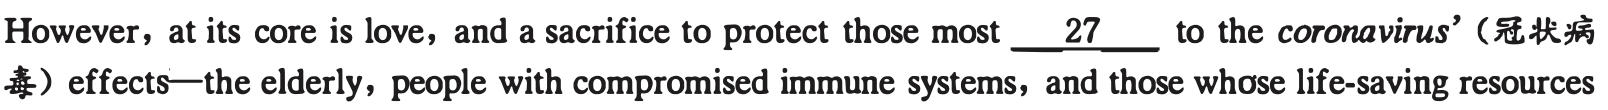
\includegraphics[width=\linewidth,height=.8\textheight,keepaspectratio]{2020-12-03.assets/char-001-line-009.png}\par

\textbf{would be used up by a} \textbf{\uline{28}} \textbf{epidemic.}


\textbf{Americans make life-saving decisions every day as a matter of course. We cut food into bite-sized} \textbf{pieces, we wear seatbelts, and we take care not to exceed the speed limit. But social distancing is}


\textbf{\uline{29}} \textbf{in that it is completely self-sacrificing. Those who will benefit may be the elderly relatives of} \textbf{the} \textbf{\uline{30}} \textbf{person we didn't pass in Starbucks, on the subway, or in the elevator.}


\textbf{Social distancing is millions of people making hundreds of sacrifices to keep the elderly alive. It} \textbf{doesn't include the - 31-- to run from . society or make an excuse to avoid one's obligations-such as} \textbf{life-saving medical work or the parental obligation to buy groceries. What it does include is applying love} \textbf{through caution. And in doing so, it offers an} \textbf{\uline{32}} \textbf{opportunity for those who care about the elderly} \textbf{to find new ways\textperiodcentered{} to love them.}


\textbf{If we're not} \textbf{\uline{33}} \textbf{as much in our normal work or school, we have extra time to call parents and}


\noindent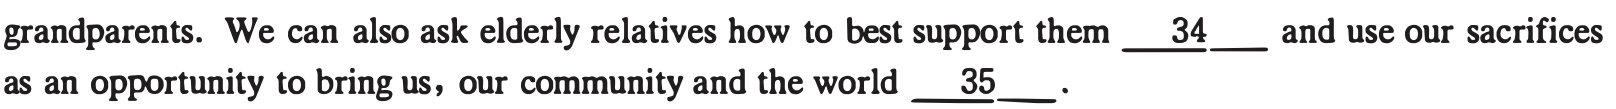
\includegraphics[width=\linewidth,height=.8\textheight,keepaspectratio]{2020-12-03.assets/char-001-line-015.png}\par

\begin{itemize}[leftmargin=2em,itemsep=.2em,topsep=.4em]\item[A.] \textbf{amazing}
\item[B.] \textbf{closer}
\item[C.] \textbf{driven}
\item[D.] \textbf{engaged}
\item[F.] \textbf{oppressing}
\item[G.] \textbf{premises}
\item[H.] \textbf{random}
\item[I.] \textbf{sentimentally}
\item[K.] \textbf{temptations}
\item[L.] \textbf{thriftier}
\item[M.] \textbf{tickled}
\item[N.] \textbf{unique}
\end{itemize}

\noindent
\includegraphics[width=\linewidth,height=.8\textheight,keepaspectratio]{2020-12-03.assets/char-001-line-017.png}\par

\subsection*{\textbf{Section B}}


\noindent
\includegraphics[width=\linewidth,height=.8\textheight,keepaspectratio]{2020-12-03.assets/char-002-line-001.png}\par

\textbf{\textit{statement contains information given in one of the paragraphs. Identify the paragraph from . which the}} \textbf{\textit{information is derived. You may choose a paragraph more than once. Each paragraph is marked with a}} \textbf{\textit{letter. Answer the questions by marking the corresponding letter on Answer Sheet 2.}}


\subsection*{\textbf{Why lifelong learning is the international imsport to success}}


A) \textbf{Picture yourself at a college graduation day, with a fresh }\textbf{\textit{cohort }}(一群)\textbf{ of students about to set sail for} \textbf{new horizons. What are they thinking while they. throw their caps in the air? What is it with this thin} \textbf{sheet of paper that makes it so precious? It's not only the proof of acquired knowledge but plays into} \textbf{the reputation game of where you were trained. Being a graduate from Harvard Law School carries} \textbf{that extra glamour, doesn't it? Yet take a closer look, and the diploma is the perfect ending to the} \textbf{modem tragedy of education.}


\noindent
\includegraphics[width=\linewidth,height=.8\textheight,keepaspectratio]{2020-12-03.assets/char-002-line-005.png}\par

\textbf{tragedy: time, action, and place. Students meet at the university campus (unity of place) for classes} \textbf{( unity of action) during their 20s ( unity of time). This classical model has traditionally produced} \textbf{prestigious universities, but it is now challenged by the digitalisation of society-which allows} \textbf{everybody who is connected to the internet to access learning-and by the need to acquire skills in step} \textbf{with a fast-changing world. Universities must realise that learning in your 20s won't be enough; If} \textbf{technological diffusion and implementation develop faster, workers will have to constantly\textperiodcentered{} refresh} \textbf{their skills.}


C) \textbf{The university model needs to evolve. It must equip students with the right skills and knowledge to} \textbf{compete in a world 'where value will be derived largely from human interaction and the ability to} \textbf{invent and interpret things that machines cannot' , as the English futurist Richard Watson puts it. By} \textbf{teaching foundational knowledge and up-to-date skills, universities wiH provide students. with the} \textbf{future-proof skills of.lifelong learning, not just get them 'job-ready'.}


D) \textbf{Some universities already play a critical role in lifelong learning as they want to keep the value of their}


\noindent
\includegraphics[width=\linewidth,height=.8\textheight,keepaspectratio]{2020-12-03.assets/char-002-line-009.png}\par

\textbf{way to start this transformation process could be to go beyond the 'five-year diploma model' to adapt} \textbf{curricula to lifelong learning. We call this model the lifelong passport.}


E) \textbf{The Bachelor's degree could be your passport to lifelong learning. For the first few years, students} \textbf{would 'learn to learn' and get endowed with reasoning skills that remain with them for the rest of} \textbf{their lives. For instance, physics allows you to observe and rationalise the world, but also to integrate}


\noindent
\includegraphics[width=\linewidth,height=.8\textheight,keepaspectratio]{2020-12-03.assets/char-002-line-012.png}\par

\textbf{predictions. Mathematics is the language used to formulate the laws of physics or economy, and to} \textbf{make rigorous computations that tum into predictions. These two disciplines natur'ally form the} \textbf{foundational pillars of education in technical universities.}


F) \textbf{Recent advances in computational methods and data science push us into rethinking science and} \textbf{engineering. Computers increasingly become principal actors in leveraging data to formulate questions,} \textbf{which requires radically new ways of reasoning. Therefore, a new discipline blending computer} \textbf{science, programming, statistics and machine learning should be added to the traditional foundational} \textbf{topics of mathematics and physics. These three pillars would allow you to keep learning complex} \textbf{technical subjects all your life because }\textbf{\textit{numeracy }}(计算)\textbf{ is the foundation upon which everything else is} \textbf{eventually built.}


G) \textbf{According to this new model, the Master of Science ( MSc) would become the first stamp in the} \textbf{lifelong learning journey. The MSc curriculum should prepare students for their professional career by} \textbf{allowing them to focus on acquiring practical skills through projects.}


H) \textbf{Those projects are then interwoven with fast-paced technical }\textbf{\textit{modules }}(模块)\textbf{ learned 'on-the-fly' and}


\textbf{'at will' depending on the nature of the project. If, for instance, your project is developing an} \textbf{integrated circuit, you will have to take a module on advanced concepts in microelectronics. The most}


\noindent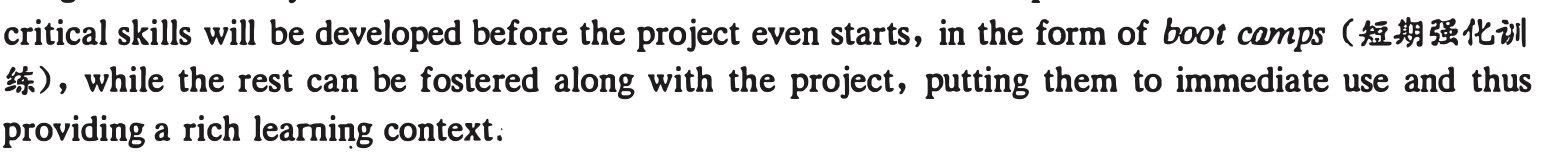
\includegraphics[width=\linewidth,height=.8\textheight,keepaspectratio]{2020-12-03.assets/char-003-line-001.png}\par

I) \textbf{In addition to technical capabilities, the very nature of projects develops social and entrepreneurial} \textbf{skills, such as design thinking, initiative taking, team leading, activity reporting or resource planning.} \textbf{Not only will those skills be actually integrated into the curriculum but they will be very important to} \textbf{have in the future because they are difficult to automate.}


J) \textbf{After the MSc diploma is earned, there would be many more stamps of lifelong learning over the} \textbf{years. If universities decide to engage in this learning model, they will have to cope with many} \textbf{organisational challenges that might shake their unity of place and action. First, the number of} \textbf{students would be unpredictable. If all of a university's }\textbf{\textit{alumni }}\raisebox{-0.225em}{
\includegraphics[height=1.05em]{2020-12-03.assets/char-003-002.png}}\allowbreak{}\raisebox{-0.225em}{
\includegraphics[height=1.05em]{2020-12-03.assets/char-003-003.png}}\allowbreak{}\raisebox{-0.225em}{
\includegraphics[height=1.05em]{2020-12-03.assets/char-003-004.png}}\allowbreak{}\textbf{ were to become students} \textbf{again, the student body would be much bigger than it is now, and it could become unsustainable for the} \textbf{campus in terms of both size and resources. Second, freshly graduated students would mix with} \textbf{professionally experienced ones. This would change the classroom dynamics, perhaps for the best.} \textbf{Project-based learning with a mixed team reflects the reality of the professional world and could} \textbf{therefore be a better preparation for it.}


K) \textbf{Sound like science fiction? In many countries, part-time studying is not exceptional: on average across} \textbf{OECD countries, part-time students in 2016 represented 20 per cent of enrolment in tertiary} \textbf{education. In many countries, this share is higher and can exceed 40 per cent in Australia,} \textbf{New Zealand and Sweden.}


L) \textbf{If lifelong learning were to become a priority and the new norm, diplomas, just like passports, could} \textbf{be revalidated periodically. A time-determined revalidation would ease administration for everybody.} \textbf{Universities as well as employers and employees would know when they have to retrain. For instance,} \textbf{graduates from the year 2000 would have to come back in 2005.}


M) \textbf{This could fix the main organisational challenges for the university, but not for the learners, due to}


\noindent
\includegraphics[width=\linewidth,height=.8\textheight,keepaspectratio]{2020-12-03.assets/char-003-line-007.png}\par

\textbf{you to save your 'travel time', but it has its limits. So far, none of the major employers associated} \textbf{with online learning platforms such as Coursera and Udacity has committed to hire or even interview} \textbf{graduates of their new online programmes.}


\noindent
\includegraphics[width=\linewidth,height=.8\textheight,keepaspectratio]{2020-12-03.assets/char-003-line-009.png}\par

\textbf{be the learner's responsibility, that of his employer, or of the state? For example, in Massachusetts,} \textbf{the healthcare professions require continuing education credits, which are carefully evidenced and} \textbf{documented. Yet the same state's lawyers don't require continuing legal education, although most} \textbf{lawyers do participate in it informally. One explanation is that technology is less of a factor in law than} \textbf{it is in healthcare.}


\textbf{0) Europe has many scenarios, but the French and Swiss ones are interesting to compare .. In France,}


\noindent
\includegraphics[width=\linewidth,height=.8\textheight,keepaspectratio]{2020-12-03.assets/char-003-line-012.png}\par

\textbf{credited as you work. In Switzerland, lifelong learning is a personal responsibility and not a} \textbf{government one. However, employers and the state encourage continuing education either by funding} \textbf{parts of it or by allowing employees to attend it.} \textbf{P) Universities have a fundamental role to play in this journey, and higher education is in for a change.}


\textbf{Just like classical theatre, the old university model produced talent and value for society. We are not} \textbf{advocating its abolition but rather calling for the adaptation of its characteristics to meet the needs of} \textbf{today.}


\textbf{36. Students should develop the key skills before they start a project.}


\textbf{37. By acquiring reasoning skills in the first few years of college, students can lay a foundation for lifelong} \textbf{learning.}


\textbf{38. The easy access to learning and rapid technological changes have brought the traditional model of} \textbf{education under challenge.}


\textbf{39. Unbelievable as it may seem, part-time students constitute a considerable portion of the student body} \textbf{in many universities across the world.}


\textbf{40. Some social and managerial skills, which are not easily automated, will be of great importance to} \textbf{students' future careers.}


\textbf{41. A new model of college education should provide students with the knowledge and skills that will make} \textbf{them more inventive and capable of lifelong learning.}


\textbf{42. A mixed student body may change the classroom dynamics and benefit learning.}


\textbf{43. The question of who will bear the cost of lifelong learning is a topic of constant debate.}


\textbf{44. To the traditional subjects of math and physics should be added a new discipline which combines} \textbf{computer science with statistics and other components.}


\textbf{45. Students who are burdened with family duties might choose to take online courses.}


\subsection*{\textbf{Section C}}


\textbf{Directions: }\textbf{\textit{There are 2 passages in this section. Each passage is followed by some questions or unfinished}} \textbf{\textit{statements. For each of them there are four choices marked }}\textbf{A), B), C) }\textbf{\textit{and }}\textbf{D). }\textbf{\textit{You should decide on the}} \textbf{\textit{best choice and mark ihe corresponding letter on Answer Sheet 2 with a single line through the centre.}}


\subsection*{\textbf{Passage One}}


\textbf{Questions 46 to SO are based on the r ollowing passage.}


\textbf{Why does social media trigger feelings of loneliness and inadequacy? Because instead of being real} \textbf{life, it is, for the most part, impression management, a way of marketing yourself, carefully choosing and} \textbf{filtering the pictures and words to put your best face forward.}


\textbf{• Online "friends" made through social \textperiodcentered{}media do not follow the normal psychological progression of an} \textbf{interpersonal relationship. You share neither physical time nor emotional conversations over the Internet.} \textbf{You simply communicate photographs and catchy posts to a diverse\textperiodcentered{} group of people whom you have} \textbf{"friended" or "followed" based on an accidental interaction. This is not to say that your social inedia} \textbf{friends can't be real friends. They absolutely can, but the two are not synonymous. Generally speaking,} \textbf{there are no unfiltered comments or casually taken photos on our social media pages. And, rightfully so,} \textbf{because it wouldn't feel safe to be completely authentic and vulnerable with some of our "friends" whom} \textbf{we don't actually know or with whom trust has yet to be built.}


\textbf{Social media can certainly be an escape from the daily grind, but we must be cautioned against the}


\noindent
\includegraphics[width=\linewidth,height=.8\textheight,keepaspectratio]{2020-12-03.assets/char-004-line-016.png}\par

\textbf{As humans, we yearn for social connection. }\textbf{\textit{Scrolling }}\textbf{O\$.\#J) through pages of pictures and comments,} \textbf{however, does not provide the same degree of fulfillment as face to face interactions do. Also, we tend to} \textbf{idealize others' lives and compare our downfalls to their greatest accomplishments, ending in feelings of} \textbf{loneliness and inadequacy.}


\textbf{Social media can lead people on the unhealthy quest for perfection. Some people begin to attend} \textbf{certain events or travel to different places so that they can snap that "perfect" photo. They begin to seek} \textbf{validation through the number of people who "like" their posts. In order for it to play a psychologically} \textbf{healthy role in your social life, social media should supplement an already healthy social network. Pictures} \textbf{and posts should be byproducts of life's treasured moments and fun times, not the planned and calculated}


\subsection*{\textbf{image that one is putting out into cyberspace in an attempt to fill insecurities or unmet needs.}}


\textbf{Ultimately, social media has increased our ability to connect with various types of people all over the} \textbf{globe. It has opened doors for businesses and allowed us to stay connected to people whom we may not} \textbf{otherwise get to follow. However, social media should feel like a fun experience, not one that contributes}


\textbf{to negative thoughts and feelings. If the latter is the case, increasing face to face time with trusted} \textbf{friends, and minimizing time scrolling online, will prove to be a reminder that your social network is much} \textbf{more rewarding than any "like," "follow" or "share" can be.}


\textbf{46. What does the author imply social media may do to our life?}


\begin{itemize}[leftmargin=2em,itemsep=.2em,topsep=.4em]\item[A.] \textbf{It may facilitate our interpersonal relationships.}
\item[B.] \textbf{It may filter our negative impressions of others.}
\item[C.] \textbf{It may make us feel isolated and incompetent.}
\item[D.] \textbf{It may render us vulnerable and inauthentic.}
\end{itemize}

\textbf{47. Why do people post comments selectively on social media?}


\begin{itemize}[leftmargin=2em,itemsep=.2em,topsep=.4em]\item[A.] \textbf{They do not find all their online friends trustworthy.}
\item[B.] \textbf{They want to avoid offending any of their audience.}
\item[C.] \textbf{They do not want to lose their followers.}
\item[D.] \textbf{They are eager to boost their popularity.}
\end{itemize}

\textbf{48. What are humans inclined to do according to the passage?}


\begin{itemize}[leftmargin=2em,itemsep=.2em,topsep=.4em]\item[A.] \textbf{Exaggerate their life's accomplishments.}
\item[B.] \textbf{Strive for perfection regardless of the cost.}
\item[C.] \textbf{Paint a rosy picture of other people's lives.}
\item[D.] \textbf{Learn lessons from other people's downfalls.}
\end{itemize}

\textbf{49. What is the author's view of pictures and posts on social media?}


\begin{itemize}[leftmargin=2em,itemsep=.2em,topsep=.4em]\item[A.] \textbf{They should record the memorable moments in people's lives.}
\item[B.] \textbf{They should be carefully edited so as to present the best image.}
\item[C.] \textbf{They should be shown in a way that meets one's security needs.}
\item[D.] \textbf{They should keep people from the unhealthy quest for perfection.}
\end{itemize}

\textbf{50. What does the author advise people to do when they find their online experience unconstructive?}


\begin{itemize}[leftmargin=2em,itemsep=.2em,topsep=.4em]\item[A.] \textbf{Use social media to increase their ability to connect with various types of people.}
\item[B.] \textbf{Stay connected to those whom they may not otherwise get to know and befriend.}
\item[C.] \textbf{Try to prevent negative thoughts and feelings from getting into the online pages.}
\item[D.] \textbf{Strengthen ties with real-life friends instead of caring about their online image.}
\end{itemize}

\subsection*{\textbf{Passage 1\textbackslash{}vo}}


\textbf{Questions 51 }\textbf{\textit{to }}\textbf{55 are based on the following passage.}


\textbf{Imagine that an alien species landed on Earth and, through their mere presence, those aliens caused} \textbf{our art to vanish, our music to homogenize, and our technological know-how to disappear. That is} \textbf{effectively what humans have been doing to our closest }\textbf{\textit{relatives-chimps }}(大猩猩)\textbf{\textit{.}}


\textbf{Back in 1999, a team of scientists led by Andrew Whiten showed that chimps from different parts of} \textbf{Africa behave very differently from one another. Some groups would get each other's attention by rapping}


\noindent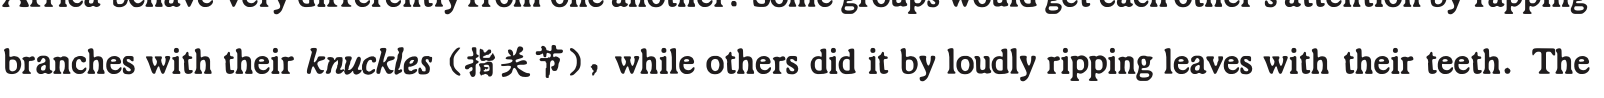
\includegraphics[width=\linewidth,height=.8\textheight,keepaspectratio]{2020-12-03.assets/char-005-line-015.png}\par

\textbf{team identified 39 of these traditions that are practiced by some communities but not others-a pattern} \textbf{that, at the time, hadn't been seen in any animal except humans. It was evidence, the team said, that} \textbf{chimps have their own cultures.}


\textbf{It took a long time to convince skeptics that such cultures exist, but now we have plenty of examples} \textbf{of animals learning local traditions from one another.}


\textbf{But just when many scientists have come to accept the existence of animal cultures, many of those} \textbf{cultures might vanish. Ammie Kalan and her colleagues have shown, through years of intensive fieldwork,} \textbf{that the very presence of humans has eroded the diversity of chimp behavior. Where we flourish, their} \textbf{cultures. wither. It is a bitterly ironic thing to learn on the 20th anniversary of Whiten's classic study.}


\textbf{"It's amazing to think that just 60 years ago, we knew next to notJ.ting of the behavior of our sister}


\noindent
\includegraphics[width=\linewidth,height=.8\textheight,keepaspectratio]{2020-12-03.assets/char-005-line-020.png}\par

\textbf{cousins, the actions of humans are closing the window on all we have discovered."}


\textbf{"Sometimes in the rush to conserve the species, I think we forget about the individuals,'' says} \textbf{Cat Hobaiter, a professor at the University of St. Andrews. "Each population, each community, even} \textbf{each generation of chimps is unique. An event might only have a small impact on the total population of} \textbf{chimps, but it may wipe out an entire community-an entire culture. No matter what we do to restore} \textbf{habitat or support population growth, we may never be able to restore that culture. "}


\textbf{No one knows whether the destruction of chimp culture is getting worse. Few places have tracked} \textbf{chimp behavior over long periods, and those that have are also more likely to have protected their animals} \textbf{from human influence.}


\textbf{Obviously conservationists need to think about saving species in a completely new way-by preserving} \textbf{animal traditions as well as bodies and genes. "Instead of focusing only on the conservation of genetically} \textbf{based entities like species, we now need to also consider culturally based entities," says Andrew Whiten.}


\textbf{51. What does the author say we humans have been doing to chimps?}


\begin{itemize}[leftmargin=2em,itemsep=.2em,topsep=.4em]\item[A.] Ruining their culture.
\item[B.] Accelerating their extinction.
\item[C.] Treating them as alien species.
\item[D.] Homogenizing their living habits.
\end{itemize}

\noindent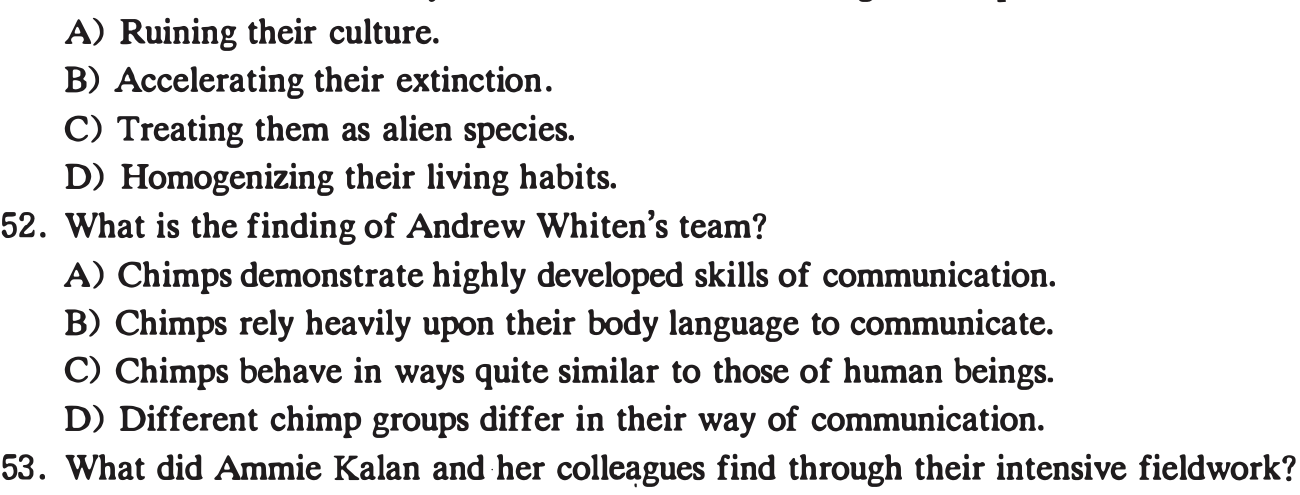
\includegraphics[width=\linewidth,height=.8\textheight,keepaspectratio]{2020-12-03.assets/char-006-line-006.png}\par

52. What is the finding of Andrew Whiten's team?


\begin{itemize}[leftmargin=2em,itemsep=.2em,topsep=.4em]\item[A.] Chimps demonstrate highly developed skills of communication.
\item[B.] Chimps rely heavily upon their body language to communicate.
\item[C.] Chimps behave in ways quite similar to those of human beings.
\item[D.] Different chimp groups differ in their way of communication.
\end{itemize}

53. What did Ammie Kalan and her colleagues find through their intensive fieldwork?


\begin{itemize}[leftmargin=2em,itemsep=.2em,topsep=.4em]\item[A.] \textbf{Whiten's classic study has little impact on the diversity of chimp behavior.}
\item[B.] \textbf{Chimp behavior becomes less varied with the increase of human activity.}
\item[C.] \textbf{Chimps alter their cµlture to quickly adapt to the changed environment.}
\item[D.] \textbf{It might already be too late to prevent animal cultures from extinction.}
\end{itemize}

\textbf{54. What does Cat Hobaiter think we should do for chimp conservation?}


\begin{itemize}[leftmargin=2em,itemsep=.2em,topsep=.4em]\item[A.] \textbf{Try to understand our sister species' behavior in the wild.}
\item[B.] \textbf{Make efforts to preserve each individual chimp community.}
\item[C.] \textbf{Study the unique characteristics\textperiodcentered{} of each generation of chimps.}
\item[D.] \textbf{Endeavor to restore chimp habitats to expand its total population.}
\end{itemize}

\textbf{55. What does the author suggest conservationists do?}


\begin{itemize}[leftmargin=2em,itemsep=.2em,topsep=.4em]\item[A.] \textbf{Focus entirely on culturally-based.entities rather than genetically-based ones.}
\item[B.] \textbf{Place more stress on animal traditions than on their physical conservation.}
\item[C.] \textbf{Conserve animal species in a novel and all-round way.}
\item[D.] \textbf{Explore the cultures of species.before they vanish.}
\end{itemize}

\textbf{Part 1V} \textbf{Translation} \textbf{( 30 minutes)}


\noindent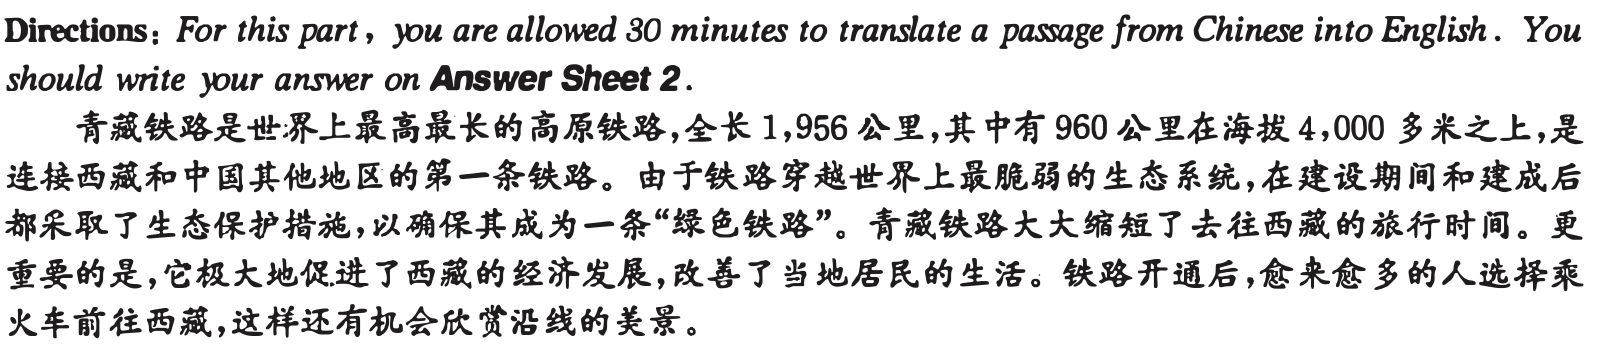
\includegraphics[width=\linewidth,height=.8\textheight,keepaspectratio]{2020-12-03.assets/char-006-line-016.png}\par
\end{document}